% ------------------------------------------------------------------------------------
%                               SISTEMI e TRASFORMAZIONI SUI SEGNALI
% ------------------------------------------------------------------------------------

\chapter{Sistemi e trasformazioni sui segnali}

Ora che abbiamo discusso cosa sono i segnali, possiamo passare alla loro elaborazione.
Per farlo, abbiamo bisogno di un \textbf{sistema}, che è banalmente:

\begin{definition}[SISTEMA]
    Un sistema è un \textbf{insieme di componenti fisici} che 
    \textbf{applica una trasformazione} ad un \textbf{segnale di ingresso} $x(t)$
    per produrre un \textbf{segnale d'uscita} $y(t)$.
\end{definition}

\begin{figure}[!ht]
    \centering
    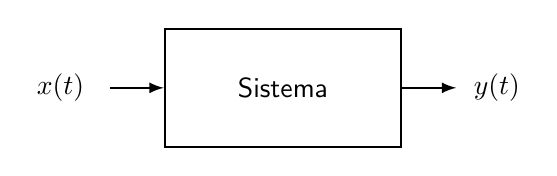
\begin{tikzpicture}[>=latex]
        \node[draw, thick, minimum width=3cm, minimum height=1.5cm] (lti) at (0,0) {\textsf{Sistema}};
        \draw[->, thick] (-2.2, 0) -- (lti.west);
        \node[anchor=east] at (-2.4, 0) {$x(t)$};
        \draw[->, thick] (lti.east) -- (2.2, 0);
        \node[anchor=west] at (2.3, 0) {$y(t)$};
    \end{tikzpicture}
    \caption{Schematizzazione di un sistema}
\end{figure}

Sostanzialmente, i sistemi sono delle \textit{"realizzazioni fisiche"} di funzioni 
che mappano segnali in altri segnali, permettondoci di \textbf{manipolarli}: combinando
componenti diverse e secondo determinati schemi possiamo \textbf{realizzare trasformazioni
"a piacimento"}.

Alcuni esempi di sistemi sono:
\begin{itemize}
    \item \textbf{FILTRI} (passa-basso, passa-alto, passa-banda)
    \item \textbf{AMPLIFICATORI}
    \item \textbf{LINEE DI TRASMISSIONE}
    \item \textbf{MICROPROCESSORI} (essenzialmente sistemi molto complessi)
\end{itemize}

Vediamo di seguito un esempio di (semplice) sistema comunemente usato: 
\begin{exa}[MEDIA MOBILE - MOVING AVERAGE]
    \[
        T: y(nT) = \frac{x(nT) + x(nT-T) + x(nT-2T)}{3}
    \] 
\end{exa}

L'output di tale sistema è la media degli ultimi tre valori del segnale discreto
in ingresso.

% ----- SISTEMI FONDAMENTALI -----

\section{Sistemi fondamentali}
\subsection{Sistemi lineari}

Particolarmente importanti sono i sistemi lineari:

\begin{definition}[SISTEMA LINEARE]
    Diciamo che un sistema $T$ è \textbf{lineare} se vale
    il \textbf{principio di sovrapposizione degli effetti}:
    \[
        T[\alpha x_{1}(t) + \beta x_{2}(t)] = \alpha T[x_{1}(t)] + \beta T[x_{2}(t)]
    \] 
\end{definition}

In altre parole, un sistema lineare rappresenta una \textbf{trasformazione lineare del segnale}
di ingresso. Attenzione al seguente esempio:

\begin{exa}[ESEMPIO FUORVIANTE]
    Il sistema caratterizzato da
    \[
        T: x(t) \mapsto y(t) = x(t-1) + 2
    \] 
    è lineare? La risposta è \textbf{no}!
\end{exa}

Infatti, considerando per esempio due segnali di ingresso $x_{1}(t)$ e $x_{2}(t)$,
abbiamo:
\[
    \begin{aligned}
        T[x_{1}(t)] &= x_{1}(t-1) + 2 \\
        T[x_{2}(t)] &= x_{2}(t-1) + 2 \\
        T[x_{1}(t) + x_{2}(t)] &= x_{1}(t-1) + x_{2}(t-1) + 2 \\ 
                               &\ne T[x_{1}(t)] + T[x_{2}(t)]
    \end{aligned}
\]
Del resto, la trasformazione applicata dal sistema è \textit{affine}, \textbf{non} \textit{lineare}.

In generale, affermiamo che:

\begin{prop}[SISTEMI LINEARI]
    I sistemi lineari sono \textbf{tutti e soli} i sistemi in
    cui il \textit{segnale di ingresso} compare nell'\textit{uscita}
    \textbf{solo} con \textbf{potenza pari a uno}.
\end{prop}

Spesso, sistemi di questo tipo possono essere scritti nella forma:
\[
    T: x(t) \mapsto y(t) = Ax(t)
\]
Dove $A$ è una matrice.
E' importante notare che le entrate di questa matrice
\textbf{non sono necessariamente costanti}.

\begin{exa}
    Il seguenee sistema è \textbf{lineare}:
    \[
        y(t) = x(t)\cos (2\pi f_{0}t)
    \] 
    Anche il seguente sistema, sebbene non sia rappresentabile in 
    forma matriciale, è \textbf{lineare}:
    \[
        y(t) = \int_{t-1}^{t} x(\tau )d \tau
    \]
\end{exa}

\subsection{Sistemi tempo invarianti}

Un'altra importante categoria di sistemi è quella dei \textbf{sistemi tempo invarianti}.

\begin{definition}[SISTEMI TEMPO INVARIANTI]
    Un sistema $T$ è detto \textbf{tempo invariante} se soddisfa:
    \[
        T[x(t)] = y(t) \implies T[x(t-t_{0})] = y(t-t_{0})
    \] 
\end{definition}

Osserviamo che il sistema \textbf{media mobile} introdotto sopra è
\textbf{tempo invariante}. Infatti, se consideriamo $x_{1}(nT)=x(nT)$ e $x_{2}(t)=x((n-n_{0})T)$ abbiamo:
\[
    \begin{aligned}
        y_{1}(nT) &= \frac{1}{3}\left[ x(nT) + x(nT-T) + x(nT-2T) \right] \\ 
        y_{2}(nT) &= \frac{1}{3}\left[ x((n-n_{0})T) + x((n-n_{0})T - T) + x((n-n_{0})T - 2T) \right] \\ 
                 &= y_{1}((n-n_{0})T)
    \end{aligned}
\]
Al contrari osserviamo, sempre su uno degli esempi visti prima:

\begin{remark}
    Il sistema $y(t)=x(t)\cos (2\pi f_{0}t)$ era \textit{lineare}, ma
    \textbf{non è tempo invariante}.
\end{remark}

Verifichiamolo per completezza, considerando $x_{1}(t) = x(t)$ e $x_{2}(t) = x(t-t_{0})$:
\[
    \begin{aligned}
        y_{1}(t) &= x(t)\cos (2\pi f_{0}t) \\ 
        y_{2}(t) &= x(t-t_{0})\cos (2\pi f_{0}t) \\ 
                 &\ne y_{1}(t-t_{0})
    \end{aligned}
\]
\begin{remark}
    Il sistema \textbf{non è tempo-invariante} perchè il \textbf{coefficiente}
    ha una \textbf{dipendenza dal tempo} $t$: lo \textit{stesso segnale}
    viene \textit{trasformato diversamente} in base all'\textit{istante
    in cui entra nel sistema}.
\end{remark}

% ----- SISTEMI CONVOLUZIONALI -----

\section{Sistemi convoluzionali}

A questo punto possiamo definire i sistemi convoluzionali:

\begin{definition}[SISTEMI LTI e CONVOLUZIONALI]
    Se un sistema è \textbf{sia lineare}, \textbf{sia tempo invariante}, è
    definito \textbf{lineare, tempo invariante}, abbreviato \textbf{LTI}.

    I \textbf{sistemi convoluzionali} (per noi) sono i \textbf{sistemi LTI}.
\end{definition}

E' opportuno notare che, in realtà, esistono \textit{"casi patologici"} di 
sistemi LTI che \textit{non sono convoluzionali}, ma noi non ce ne occuperemo.

In ogni caso, tali sistemi sono detti convoluzionali per il seguente motivo:

\begin{prop}[SISTEMI CONVOLUZIONALI]
    Dato un sistema convoluzionale, la sua \textbf{risposta} $y(t)$
    ad un \textbf{ingresso} $x(t)$ è esprimibile come segue:
    \[
        y(t) = x(t) \ast h(t)
    \] 
    Cioè la risposta è data dall \textbf{convoluzione} tra l'\textbf{ingresso}
    $x(t)$ e la \textbf{risposta impulsiva} $h(t)$, che è \textit{caratteristica} 
    del sistema.
\end{prop}

\begin{figure}[!ht]
    \centering
    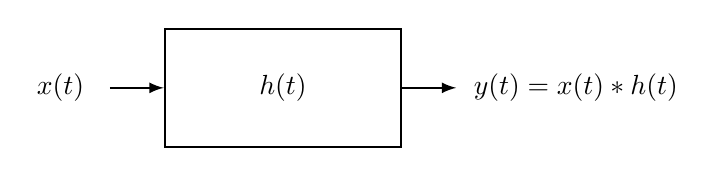
\begin{tikzpicture}[>=latex]
        \node[draw, thick, minimum width=3cm, minimum height=1.5cm] (lti) at (0,0) {$h(t)$};
        \draw[->, thick] (-2.2, 0) -- (lti.west);
        \node[anchor=east] at (-2.4, 0) {$x(t)$};
        \draw[->, thick] (lti.east) -- (2.2, 0);
        \node[anchor=west] at (2.3, 0) {$y(t) = x(t)\ast h(t)$};
    \end{tikzpicture}
    \caption{Schematizzazione di un sistema convoluzionale}
\end{figure}

\subsection{Convoluzione}

Per capire meglio di cosa stiamo parlando, definiamo l'operazione
di convoluzione:

\begin{definition}[CONVOLUZIONE]
    Date due funzioni $x(t)$ e $y(t)$, la loro \textbf{convoluzione} è
    definita come segue:
    \[
        z(t) = x(t) \ast y(t) = \int_{-\infty}^{+\infty} x(\tau )y(t-\tau )d\tau
    \] 
\end{definition}

\subsection{Proprietà della convoluzione}

Elenchiamo di seguito alcune proprietà utili delle convoluzioni:
\begin{enumerate}
    \item \textbf{COMMUTATIVITA'}: $f\ast g = g\ast f$.
    \item \textbf{ASSOCIATIVITA'}: $f\ast (g \ast h) = .(f\ast g)\ast h$
    \item \textbf{DISTRIBUTIVITA'} (rispetto alla somma): $f\ast (g+h) = (f\ast g) + (f\ast h)$.
\end{enumerate}

Sono utili anche i seguenti fatti:
\begin{enumerate}
    \item L'area del segnale $z(t)$ è uguale al \textbf{prodotto delle aree}.
    \item La durata del segnale $z(t)$ è uguale alla \textbf{somma delle durate}.
\end{enumerate}

\subsection{Impulso di Dirac}

L'elemento neutro per la convoluzione è l'impulso di Dirac:

\begin{definition}[IMPULSO DI DIRAC]
    \[
        \delta(t) \coloneqq \begin{cases}
            0 & \forall t\ne 0 \\ 
            +\infty & t = 0
        \end{cases}
    \]
\end{definition}

\begin{figure}
    \centering
    \begin{tikzpicture}[scale = 0.8]
        \begin{axis}[
            width=10cm,
            height=8cm,
            xmin=-2.1, xmax=2.1,
            ymin=-0.25, ymax=1.25,
            xtick={-2,-1,0,1,2},
            minor x tick num=4, 
            ytick={-0.2, 0.0, 0.2, 0.4, 0.6, 0.8, 1.0, 1.2},
            yticklabel style={
                /pgf/number format/fixed,
                /pgf/number format/precision=1
            },
            minor y tick num=1,
            xlabel={x},
            tick align=inside,
            axis on top,
            thick,
            tick style={thick, black}
            ]
            \draw[nord11, thick] (axis cs:-2.1,0) -- (axis cs:2.1,0);
            \draw[nord11, thick, ->, >=stealth, shorten <= 3pt] (axis cs:0,0) -- (axis cs:0,1);
            \addplot[nord11, thick, mark=*, 
                mark options={fill=white, scale=1.2}, only marks] coordinates {(0,0)};

        \end{axis}
    \end{tikzpicture}
    \caption{Impulso di Dirac}
\end{figure}

E' importante notare che vale:
\[
    \text{Area}[\delta(t)] = \int_{-\infty}^{+\infty}\delta(t) dt = 1    
\] 

\begin{prop}[ELEMENTO NEUTRO PER LA CONVOLUZIONE]
    L'impulso di Dirac è l'elemento neutro per la convoluzione.
    Dato un segnale $x(t)$, abbiamo:
    \[
        \begin{aligned}
            x(t) \ast \delta(t) &= x(t) \\ 
            x(t) \ast \delta(t-t_{0}) &= x(t-t_{0})
        \end{aligned}
    \] 
\end{prop}

In particolare, è importante la \textbf{proprietà rivelatrice
dell'impulso}, che, come suggerito dal nome, \textit{"mette in evidenza"} il valore del segnale
al tempo specificato.

\begin{prop}[PROPRIETA' RIVELATRICE DELL'IMPULSO]
    \[
        \begin{aligned}
            x(t) \delta(t-t_{0}) &= x(t_{0}) \delta(t-t_{0}) \\ 
            \int_{-\infty}^{+\infty} x(t) \delta(t-t_{0}) dt &= x(t_{0})
        \end{aligned}
    \] 
\end{prop}

Inoltre, vale il seguente fatto:

\begin{prop}[SISTEMI LTI E IMPULSO DI DIRAC]
    Dato un \textbf{sistema LTI}, se questo riceve come ingresso un segnale
    \[
        x_{\text{in}}(t) = \delta(t) 
    \] 
    la sua \textbf{uscita} sarà la \textbf{risposta impulsiva} $h(t)$ del sistema.
\end{prop}

\subsection{Esempi di calcolo delle convoluzioni}

Facciamo un esempio:

\begin{exa}[ESEMPIO CONVOLUZIONE]
    Consideriamo i seguenti due segnali:
    \[
        \begin{aligned}
            x(t) &= \text{rect}\left( \frac{t-1}{6} \right) \\ 
            y(t) &= e^{-\alpha t} \text{ , } \alpha\in \mathbb{R}^+
        \end{aligned}
    \] 
    Calcoliamo:
    \[
        z(t) = \int_{-\infty}^{+\infty} y(\tau )x(t-\tau )d\tau
    \]
    Per quanto detto sopra sulla durata, ci aspettiamo:
    \[
        z(t) \ne 0 \Leftrightarrow t\in [-2,+\infty)
    \]
    Intanto, abbiamo:
    \[
        \begin{aligned}
            y(\tau ) &= e^{-\alpha \tau } \\ 
            x(t-\tau ) &= \text{rect}\left( \frac{t-\tau -1}{6} \right)
        \end{aligned}
    \] 
    Ora, procediamo per casi (illustrati nella figura~\ref{fig:03_01_convoluzione_esempio}):

    \paragraph{I $t\le -2$} Qui non vi è nessuna sovrapposizione tra $x(t-\tau )$
    e $y(\tau )$.

    \paragraph{II $-2<t<4$} Qui il rettangolo inizia a sovrapporsi al secondo 
    segnale (ma la sovrapposizione è solo parziale). Abbiamo quindi:
    \[
        \begin{aligned}
            z(t) &= \int_{0}^{t+2} \underbrace{ \text{rect}(\ldots ) }_{=1} e^{-\alpha \tau }d\tau \\
            &=\frac{1}{\alpha}\left[ 1 - e^{\alpha(t+2)} \right] 
        \end{aligned}
    \] 
    \paragraph{III $t\ge 4$} Qui il rettangolo si sovrappone del tutto con il secondo segnale.
    \[
        \begin{aligned}
            z(t) &= \int_{t-4}^{t+2} \underbrace{ \text{rect}(\ldots ) }_{=1} e^{-\alpha \tau }d\tau \\ 
                 &=\frac{1}{\alpha}e^{-\alpha t}[e^{4 \alpha} - e^{-2 \alpha}] 
        \end{aligned}
    \] 

    Per cui concludiamo che il risultato complessivo è:
    \[
        z(t) = \begin{cases}
            0 & t \le  -2 \\ 
            \frac{1}{\alpha}\left[ 1 - e^{\alpha(t+2)} \right] & -2 < t < -4 \\ 
            \frac{1}{\alpha}e^{-\alpha t}[e^{4 \alpha} - e^{-2 \alpha}] & t\ge 4
        \end{cases}
    \] 
\end{exa}

\begin{figure}[!ht]
    \centering

    % --- CASO 1: Sovrapposizione nulla ---
    \begin{tikzpicture}
        \begin{axis}[
            width=0.85\textwidth, height=4cm,
            axis lines=middle, xlabel={\(\tau\)}, ylabel={},
            xmin=-8, xmax=9, ymin=-0.1, ymax=1.5,
            xtick={-8,-6,-4,-2,0,2,4,6,8},
            ytick={0, 1},
            grid=major, grid style={dashed, nord3!30},
            axis line style={nord0}, tick style={nord0}, tick label style={color=nord0},
            xlabel style={below right, color=nord0}
            ]
            % Segnale y(tau)
            \addplot[thick, nord10, domain=0:9, samples=100] {exp(-0.5*x)};
            \node[nord10, anchor=south] at (axis cs: 2, 0.6) {\(y(\tau)\)};

            % Segnale x(t-tau) con t = -3 (rettangolo da -7 a -1)
            \addplot[thick, nord11] coordinates { (-7,0) (-7,1) (-1,1) (-1,0) };
            \node[nord11, anchor=south] at (axis cs: -4, 1.05) {\(x(t-\tau)\)};

        \end{axis}
    \end{tikzpicture}

    \vspace{0.4cm} % Spazio tra le figure

    % --- CASO 2: Sovrapposizione parziale ---
    \begin{tikzpicture}
        \begin{axis}[
            width=0.85\textwidth, height=4cm,
            axis lines=middle, xlabel={\(\tau\)}, ylabel={},
            xmin=-8, xmax=9, ymin=-0.1, ymax=1.5,
            xtick={-8,-6,-4,-2,0,2,4,6,8},
            ytick={0, 1},
            grid=major, grid style={dashed, nord3!30},
            axis line style={nord0}, tick style={nord0}, tick label style={color=nord0},
            xlabel style={below right, color=nord0}
            ]
            % Area di sovrapposizione (da 0 a t+2 = 3)
            \addplot[fill=nord8!30, draw=none, domain=0:3, samples=100] {exp(-0.5*x)} \closedcycle;

            % Segnale y(tau)
            \addplot[thick, nord10, domain=0:9, samples=100] {exp(-0.5*x)};
            \node[nord10, anchor=south] at (axis cs: 4.5, 0.6) {\(y(\tau)\)};

            % Segnale x(t-tau) con t = 1 (rettangolo da -3 a 3)
            \addplot[thick, nord11] coordinates { (-3,0) (-3,1) (3,1) (3,0) };
            \node[nord11, anchor=south] at (axis cs: 0, 1.05) {\(x(t-\tau)\)};

        \end{axis}
    \end{tikzpicture}

    \vspace{0.4cm} % Spazio tra le figure

    % --- CASO 3: Sovrapposizione totale ---
    \begin{tikzpicture}
        \begin{axis}[
            width=0.85\textwidth, height=4cm,
            axis lines=middle, xlabel={\(\tau\)}, ylabel={},
            xmin=-8, xmax=9, ymin=-0.1, ymax=1.5,
            xtick={-8,-6,-4,-2,0,2,4,6,8},
            ytick={0, 1},
            grid=major, grid style={dashed, nord3!30},
            axis line style={nord0}, tick style={nord0}, tick label style={color=nord0},
            xlabel style={below right, color=nord0}
            ]
            % Area di sovrapposizione (da t-4=1 a t+2=7)
            \addplot[fill=nord8!30, draw=none, domain=1:7, samples=100] {exp(-0.5*x)} \closedcycle;

            % Segnale y(tau)
            \addplot[thick, nord10, domain=0:9, samples=100] {exp(-0.5*x)};
            \node[nord10, anchor=south] at (axis cs: 2.5, 0.3) {\(y(\tau)\)};

            % Segnale x(t-tau) con t = 5 (rettangolo da 1 a 7)
            \addplot[thick, nord11] coordinates { (1,0) (1,1) (7,1) (7,0) };
            \node[nord11, anchor=south] at (axis cs: 4, 1.05) {\(x(t-\tau)\)};

        \end{axis}
    \end{tikzpicture}

    \caption{Illustrazione dei tre casi: sovrapposizione nulla, parziale e totale.}
    \label{fig:03_01_convoluzione_esempio}
\end{figure}

E' utile anche considerare il seguente risultato:

\begin{prop}[CONVOLUZIONE TRA DUE RETTANGOLI]
    Consideriamo due funzioni rettangolo:
    \[
        \begin{aligned}
            x(t) &= A \text{rect}\left( \frac{t}{T} \right) \\ 
            y(t) &= B \text{rect} \left( \frac{t}{T} \right)
        \end{aligned}
    \] 
    La loro convoluzione è:
    \[
        z(t) = x(t) \ast y(t) = kAB \text{triang} \left( \frac{t}{T} \right)
    \]
\end{prop}

Possiamo determinare il parametro $k$ semplicemente sfruttando la proprietà delle convoluzioni
sull'area del segnale risultante:
\[
    \begin{aligned}
        \text{Area}[x(t)] &= AT \\ 
        \text{Area}[y(t)] &= BT \\ 
        \text{Area}[z(t)] &= kABT \coloneqq ABT^2 \implies k=T
    \end{aligned}
\]
\subsection{Convoluzione in tempo discreto}

A tempo discreto, la definizione di convoluzione diventa:

\begin{definition}[CONVOLUZIONE A TEMPO DISCRETO]
    Dati due segnali $x(nT)$ e $y(nT)$, la loro convoluzione è definita come:
    \[
        z(nT) = x(nT) \ast y(nT) \coloneqq T\sum_{k=-\infty}^\infty x(kT)y(nT-kT)
    \] 
\end{definition}
